\documentclass[tikz]{standalone}

\begin{document}
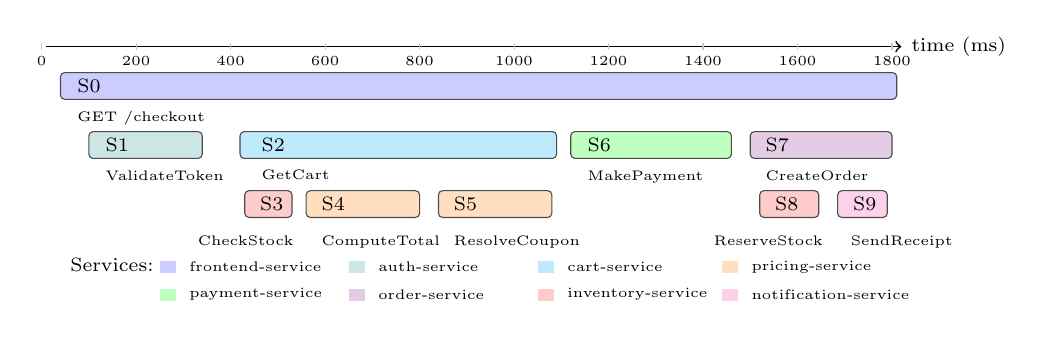
\begin{tikzpicture}[
  x=0.6cm,
  y=0.5cm,
  span/.style={rounded corners=1.5pt, draw=black!70, line width=0.5pt, minimum height=0.48cm, align=left, font=\scriptsize,}
]

% One color per service to ease visual tracking across spans
\colorlet{svcFront}{blue!20}
\colorlet{svcAuth}{teal!20}
\colorlet{svcCart}{cyan!25}
\colorlet{svcPricing}{orange!25}
\colorlet{svcPayment}{green!25}
\colorlet{svcOrder}{violet!20}
\colorlet{svcInventory}{red!20}
\colorlet{svcNotify}{magenta!18}

% Time axis
\draw[->, line width=0.6pt] (0.1,1) -- (18.2,1) node[anchor=west, font=\scriptsize] {time (ms)};
\foreach \t in {0,2,...,18} {
  \draw[gray!45] (\t,1.08) -- (\t,0.92);
  \pgfmathtruncatemacro{\ms}{100*\t}
  \node[font=\tiny, anchor=north] at (\t,1) {\ms};
}

% Span bars: vertical position encodes call-tree depth
\draw[fill=svcFront, draw=black!70, rounded corners=1.5pt] (0.4,-0.34) rectangle (18.10,0.34);
\node[font=\scriptsize, anchor=west] at (0.55,0) {S0};
\node[font=\tiny, anchor=north west] at (0.55,-0.40) {GET /checkout};

\draw[fill=svcAuth, draw=black!70, rounded corners=1.5pt] (1.0,-1.84) rectangle (3.4,-1.16);
\node[font=\scriptsize, anchor=west] (S1) at (1.15,-1.5) {S1};
\node[font=\tiny, anchor=north west] at (1.15,-1.90) {ValidateToken};

\draw[fill=svcCart, draw=black!70, rounded corners=1.5pt] (4.2,-1.84) rectangle (10.9,-1.16);
\node[font=\scriptsize, anchor=west] (S2) at (4.45,-1.5) {S2};
\node[font=\tiny, anchor=north west] at (4.45,-1.90) {GetCart};

\draw[fill=svcPayment, draw=black!70, rounded corners=1.5pt] (11.2,-1.84) rectangle (14.6,-1.16);
\node[font=\scriptsize, anchor=west] (S6) at (11.35,-1.5) {S6};
\node[font=\tiny, anchor=north west] at (11.35,-1.90) {MakePayment};

\draw[fill=svcOrder, draw=black!70, rounded corners=1.5pt] (15.0,-1.84) rectangle (18.0,-1.16);
\node[font=\scriptsize, anchor=west] (S7) at (15.12,-1.5) {S7};
\node[font=\tiny, anchor=north west] at (15.12,-1.90) {CreateOrder};

\draw[fill=svcInventory, draw=black!70, rounded corners=1.5pt] (4.30,-3.34) rectangle (5.30,-2.66);
\node[font=\scriptsize, anchor=west] (S3) at (4.42,-3.0) {S3};
\node[font=\tiny, anchor=north west] at (3.10,-3.56) {CheckStock};

\draw[fill=svcPricing, draw=black!70, rounded corners=1.5pt] (5.60,-3.34) rectangle (8.00,-2.66);
\node[font=\scriptsize, anchor=west] (S4) at (5.72,-3.0) {S4};
\node[font=\tiny, anchor=north west] at (5.72,-3.56) {ComputeTotal};

\draw[fill=svcInventory, draw=black!70, rounded corners=1.5pt] (15.20,-3.34) rectangle (16.45,-2.66);
\node[font=\scriptsize, anchor=west] (S8) at (15.32,-3.0) {S8};
\node[font=\tiny, anchor=north west] at (14.02,-3.56) {ReserveStock};

\draw[fill=svcNotify, draw=black!70, rounded corners=1.5pt] (16.85,-3.34) rectangle (17.90,-2.66);
\node[font=\scriptsize, anchor=west] (S9) at (16.97,-3.0) {S9};
\node[font=\tiny, anchor=north west] at (16.92,-3.56) {SendReceipt};

\draw[fill=svcPricing, draw=black!70, rounded corners=1.5pt] (8.40,-3.34) rectangle (10.80,-2.66);
\node[font=\scriptsize, anchor=west] (S5) at (8.52,-3.0) {S5};
\node[font=\tiny, anchor=north west] at (8.52,-3.56) {ResolveCoupon};

% Legend (service colors) - wider columns and clearer vertical spacing
\node[font=\scriptsize, anchor=west] at (0.4,-4.55) {Services:};

\fill[svcFront] (2.5,-4.75) rectangle (2.85,-4.45);
\node[font=\tiny, anchor=west] at (2.92,-4.60) {frontend-service};
\fill[svcAuth] (6.5,-4.75) rectangle (6.85,-4.45);
\node[font=\tiny, anchor=west] at (6.92,-4.60) {auth-service};
\fill[svcCart] (10.5,-4.75) rectangle (10.85,-4.45);
\node[font=\tiny, anchor=west] at (10.92,-4.60) {cart-service};
\fill[svcPricing] (14.4,-4.75) rectangle (14.75,-4.45);
\node[font=\tiny, anchor=west] at (14.82,-4.60) {pricing-service};

\fill[svcPayment] (2.5,-5.45) rectangle (2.85,-5.15);
\node[font=\tiny, anchor=west] at (2.92,-5.30) {payment-service};
\fill[svcOrder] (6.5,-5.45) rectangle (6.85,-5.15);
\node[font=\tiny, anchor=west] at (6.92,-5.30) {order-service};
\fill[svcInventory] (10.5,-5.45) rectangle (10.85,-5.15);
\node[font=\tiny, anchor=west] at (10.92,-5.30) {inventory-service};
\fill[svcNotify] (14.4,-5.45) rectangle (14.75,-5.15);
\node[font=\tiny, anchor=west] at (14.82,-5.30) {notification-service};

\end{tikzpicture}
\end{document}
